\section{Introduction}

\begin{frame}<beamer>{Outline}
    \tableofcontents[currentsection,currentsubsection]
\end{frame}
  
\begin{frame}{Introduction}
    
    \begin{itemize}
    	\item How to learn to classify objects from images?
        \item What algorithms to use?
        \item How to scale up these algorithms?
	\end{itemize}
 
	\begin{figure}[!tbp]
	  \centering
	  %\begin{minipage}[b]{0.4\textwidth}
	    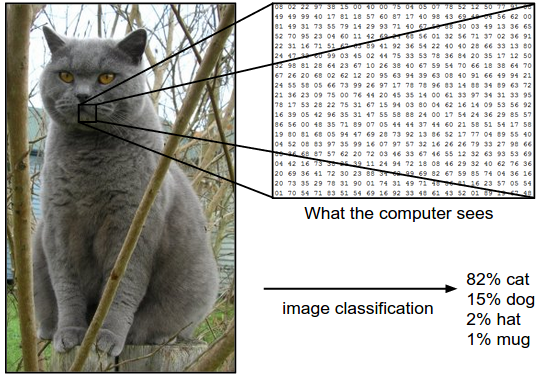
\includegraphics[width=0.5\textwidth]{classify.png}
	  %\end{minipage}
	\end{figure}

\end{frame}

\begin{frame}{Classification}

	\begin{itemize}
	\item Dataset $\mathcal{D} = \{x^{(i)},y^{(i)}\}_{i=1:N}$ with $x^{(i)} \in \mathbb{R}^D$ and labels $y^{(i)} \in \mathbb{R}^P$
	\item Make accurate prediction $\hat{y}$ on unseen data point $x$	
	\item Classifier (parameters $\theta$) approximates label as: $y \approx \hat{y} = F(x; \theta)$	
	\item Classifier learns parameters ($\theta$) from data $\mathcal{D}$ to minimize a pre-specified loss function
	\end{itemize}

\end{frame}

\begin{frame}{Neuron}

	\begin{figure}[!tbp]
	%\centering
	\begin{minipage}[b]{0.4\textwidth}
    	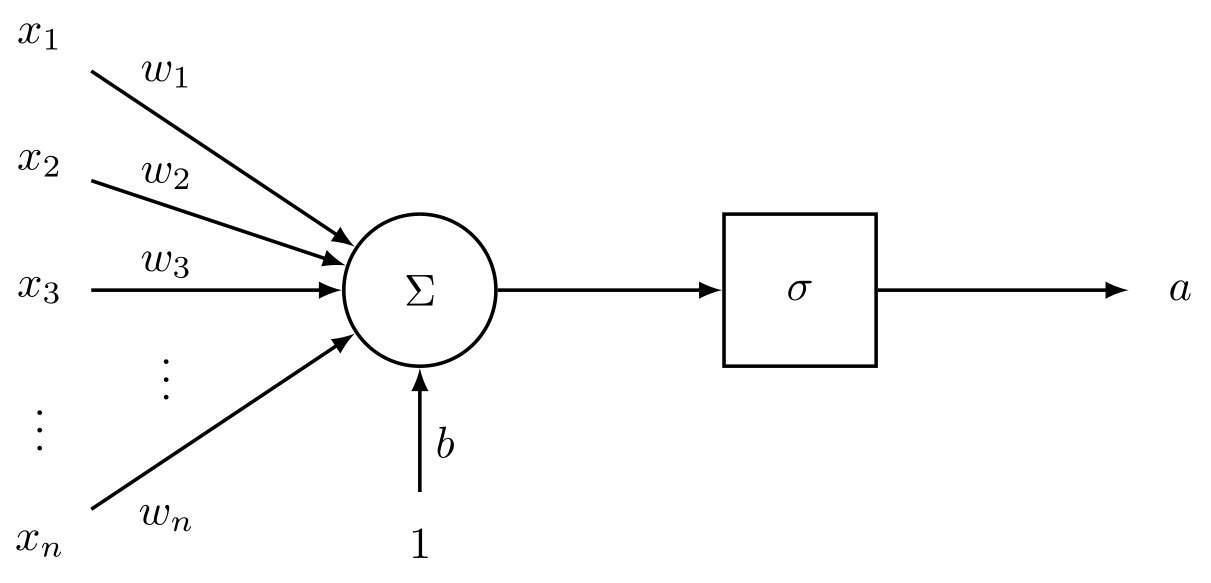
\includegraphics[width=2in]{neuron.png}
  	\end{minipage}
  	%\hfill
  	\begin{minipage}[b]{0.4\textwidth}
    	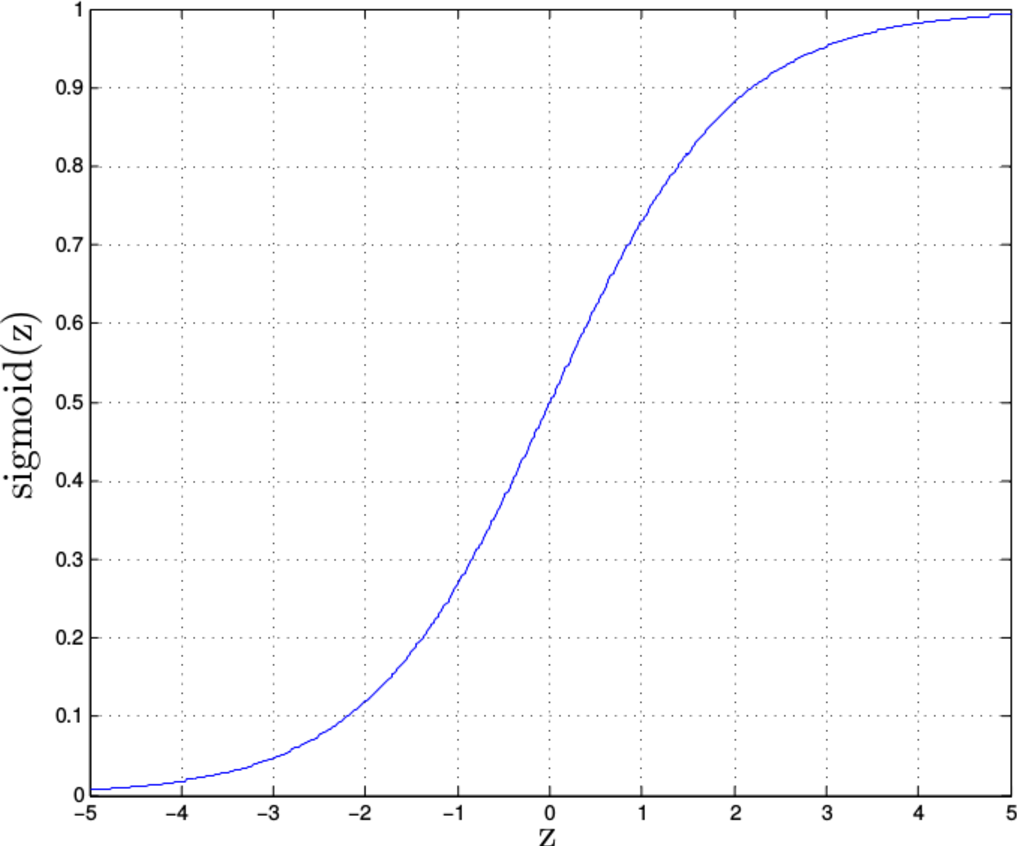
\includegraphics[width=2in]{sigmoid.pdf}
  	\end{minipage}
	\end{figure}
	
	\begin{align*}
	a = f(w^T x + b)
	\end{align*}
	
	\begin{itemize}
	\item $w \in \mathbb{R}^n = $ Weight vector
	\item $b \in \mathbb{R} = $ Scalar bias
	\end{itemize} 

\end{frame}

\begin{frame}{Classifier: Neural Network}

	\begin{figure}[!tbp]
	  \centering
	    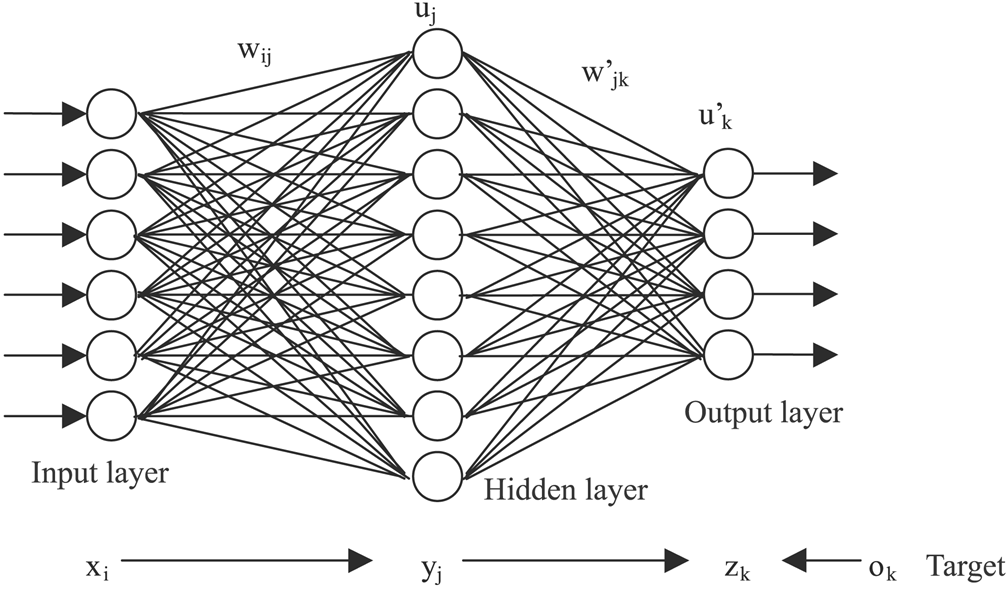
\includegraphics[width=0.6\textwidth]{nnet.png}
	\end{figure}
	
	For each layer,
	\begin{align*}
	z_l = (W_l)^T x_l + b_l; \hspace{16pt}
	a_l = f(z_l)
	\end{align*}
	
	\begin{itemize}
	\item $W^l \in \mathbb{R}^{n_{l-1} \times n_l} = $ Weight vector
	\item $b_l \in \mathbb{R}^{n_l} = $ Scalar bias
	\end{itemize} 

\end{frame}